% CVPR 2027 Paper Template; see https://github.com/cvpr-org/author-kit
% Built from the official author kit (author-kit-CVPR2027-v1-latex.zip, kept in _kit_download/).

\documentclass[10pt,twocolumn,letterpaper]{article}

%%%%%%%%% PAPER TYPE  - PLEASE UPDATE FOR FINAL VERSION
% \usepackage{cvpr}              % To produce the CAMERA-READY version
\usepackage[review]{cvpr}      % To produce the REVIEW version
% \usepackage[pagenumbers]{cvpr} % To force page numbers, e.g. for an arXiv version

% Import additional packages in the preamble file, before hyperref
% Shared by main.tex and supplement.tex. Standard CVPR geometry is unchanged.
\usepackage[T1]{fontenc}
\usepackage{times}
\usepackage{amsmath,amssymb}
\usepackage{booktabs,multirow}
\usepackage{microtype}
\usepackage{algorithm}
\usepackage{algpseudocode}
\usepackage{xspace}
\newcommand{\ours}{\mbox{SE-JEPA}\xspace}
\newcommand{\base}{\theta_0}
\newcommand{\memory}{\mathcal{M}}
\newcommand{\replay}{\mathcal{R}}
\newcommand{\loss}{\mathcal{L}}
\newcommand{\R}{\mathbb{R}}
\DeclareMathOperator*{\argmin}{arg\,min}
\DeclareMathOperator*{\argmax}{arg\,max}
\newcommand{\missing}{\textemdash}
\newcommand{\best}[1]{\textbf{#1}}
\newcommand{\supref}[1]{Appendix~#1}
% References from the appendix to main-paper labels (supplement.tex redefines this for xr).
\providecommand{\mainref}[1]{\ref{#1}}
\hyphenation{AdaJEPA}
\setcounter{dbltopnumber}{2}
\graphicspath{{figures/}}
% Primitive input keeps LaTeX file hooks out of tabular alignment rows.
\makeatletter
\newcommand{\inputrows}[1]{\@@input #1 }
\makeatother

% Keep figure-only review pages aligned to the top.
\makeatletter
\setlength{\@fptop}{0pt}
\setlength{\@dblfptop}{0pt}
\makeatother


% It is strongly recommended to use hyperref, especially for the review version.
% hyperref with option pagebackref eases the reviewers' job.
\definecolor{cvprblue}{rgb}{0.21,0.49,0.74}
\usepackage[pagebackref,breaklinks,colorlinks,allcolors=cvprblue]{hyperref}

\def\confName{CVPR}
\def\confYear{2027}

%%%%%%%%% TITLE (set by the authors on 2026-10-30)
\title{SE-JEPA: Self-Evolving Latent World Models}

%%%%%%%%% AUTHORS - hidden in review mode; fill in for the camera-ready version
\author{Anonymous CVPR submission}

\begin{document}
\maketitle
\begin{abstract}
\looseness=-1
We propose \ours{}, a framework that turns deployment experience into reusable predictive knowledge, enabling world models to learn continually under recurring environmental changes. The method decouples fast within-episode adaptation from cross-episode learning, building predictive capabilities by replaying observed interaction trajectories rather than directly inheriting episode-specific weight updates. \ours{} automatically groups predictively compatible trajectories into predictive domains and trains a separate slow predictor for each domain in a fixed representation space. Prediction errors guide experience selection and predictor validation, while current interactions determine which predictor to use for planning. The framework requires neither predefined domain labels nor domain-switch signals and supports both gradient-based and sampling-based planners. Experiments show that \ours{} improves test success over AdaJEPA by 15.4--17.1 percentage points on PushObj shapes unseen during pretraining and 15.9--18.7 points on PushT visual shifts. In a repeated-goal stream spanning 14 shape and visual conditions, online success increases from 65.3\% to 75.5\% over five deployment rounds. Furthermore, with DINO-WM as the backbone, a predictor trained through a single consolidation pass reduces Chamfer distance by 47\% on rope instances excluded from learning, without within-episode adaptation. These results demonstrate that \ours{} not only corrects current predictions but also enables world models to continually improve subsequent planning. The source code will be made publicly available.

% Latent world models enable action planning but struggle with distribution shifts after deployment. Test-time adaptation addresses these shifts within an episode, yet resets afterward, forcing agents to repeatedly relearn recurring changes. We find that carrying adapted weights forward fails: consecutive updates are nearly orthogonal (mean cosine 0.018), and inheriting them cuts success from 62\% to 48\%. We therefore retain the observed transitions, not the weight updates. Inspired by complementary learning systems, we propose \ours{}, which pairs fast within-episode adaptation with slow cross-episode consolidation. The original pretrained weights remain fixed, while a separate slow predictor for each self-discovered domain learns from replayed trajectories. Its own prediction errors guide what to store and when to trust a learned predictor. No shift labels or task boundaries are needed, and both gradient-based and sampling-based planners benefit. \ours{} achieves state-of-the-art results, improving held-out success over AdaJEPA by 15.4--17.1 percentage points on unseen PushObj shapes and 15.9--18.7 points on PushT visual shifts. Relative to pretrained DINO-WM, it reduces Chamfer distance by 48.6\% on rope and 26.7\% on granular, with continued gains over deployment. The source code~will~be~made~public.
\end{abstract}


\section{Introduction}
\label{sec:intro}

\begin{figure}[t]
  \centering
  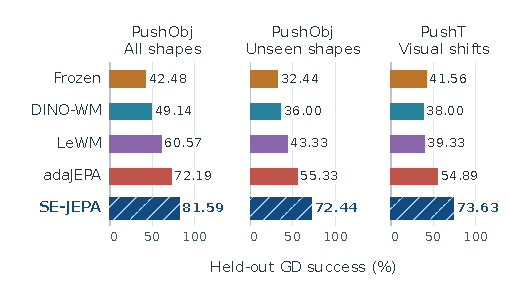
\includegraphics[width=\linewidth]{teaser_bars.pdf}
  \caption{\textbf{Deployment experience improves held-out planning.} Held-out success with CEM planning on PushObj shapes, the three shapes unseen during pretraining, and six PushT visual shifts.}
  \label{fig:teaser_bars}
\end{figure}

World models let an agent try actions in imagination before committing to them. Latent world models make this practical for visual control: they predict how an encoded scene evolves under candidate actions, and a model-predictive controller (MPC) searches for the action sequence whose predicted outcome matches an image goal~\cite{zhou2024dinowm,wang2026straightening,maes2026lewm}. Planning is only as good as these predictions. When a deployed agent meets an object shape or a visual appearance it was not trained on, prediction errors turn directly into planning failures.

Test-time adaptation offers a remedy. AdaJEPA~\cite{wang2026adajepa} treats every executed action as free supervision: the observed transition corrects the predictor before the next replan. This closes a second feedback loop around MPC and recovers much of the lost performance within an episode. The correction, however, is discarded when the episode ends. An agent that pushes the same unfamiliar object a hundred times relearns its dynamics a hundred times.

We ask whether a world model can instead \emph{remember} what it learns during deployment. The key is to turn local corrections into reusable predictions. A fast update fits a short trajectory around one start and goal; across episodes, these updates point in nearly orthogonal directions. Directly retaining them does not reliably produce a predictor that serves the full stream. On a matched stream, full accumulation lowers success from 62\% to 48\% (Sec.~\ref{sec:diagnosis}). What should persist is the experience behind an update, not the update itself.

\begin{figure*}[t]
  \centering
  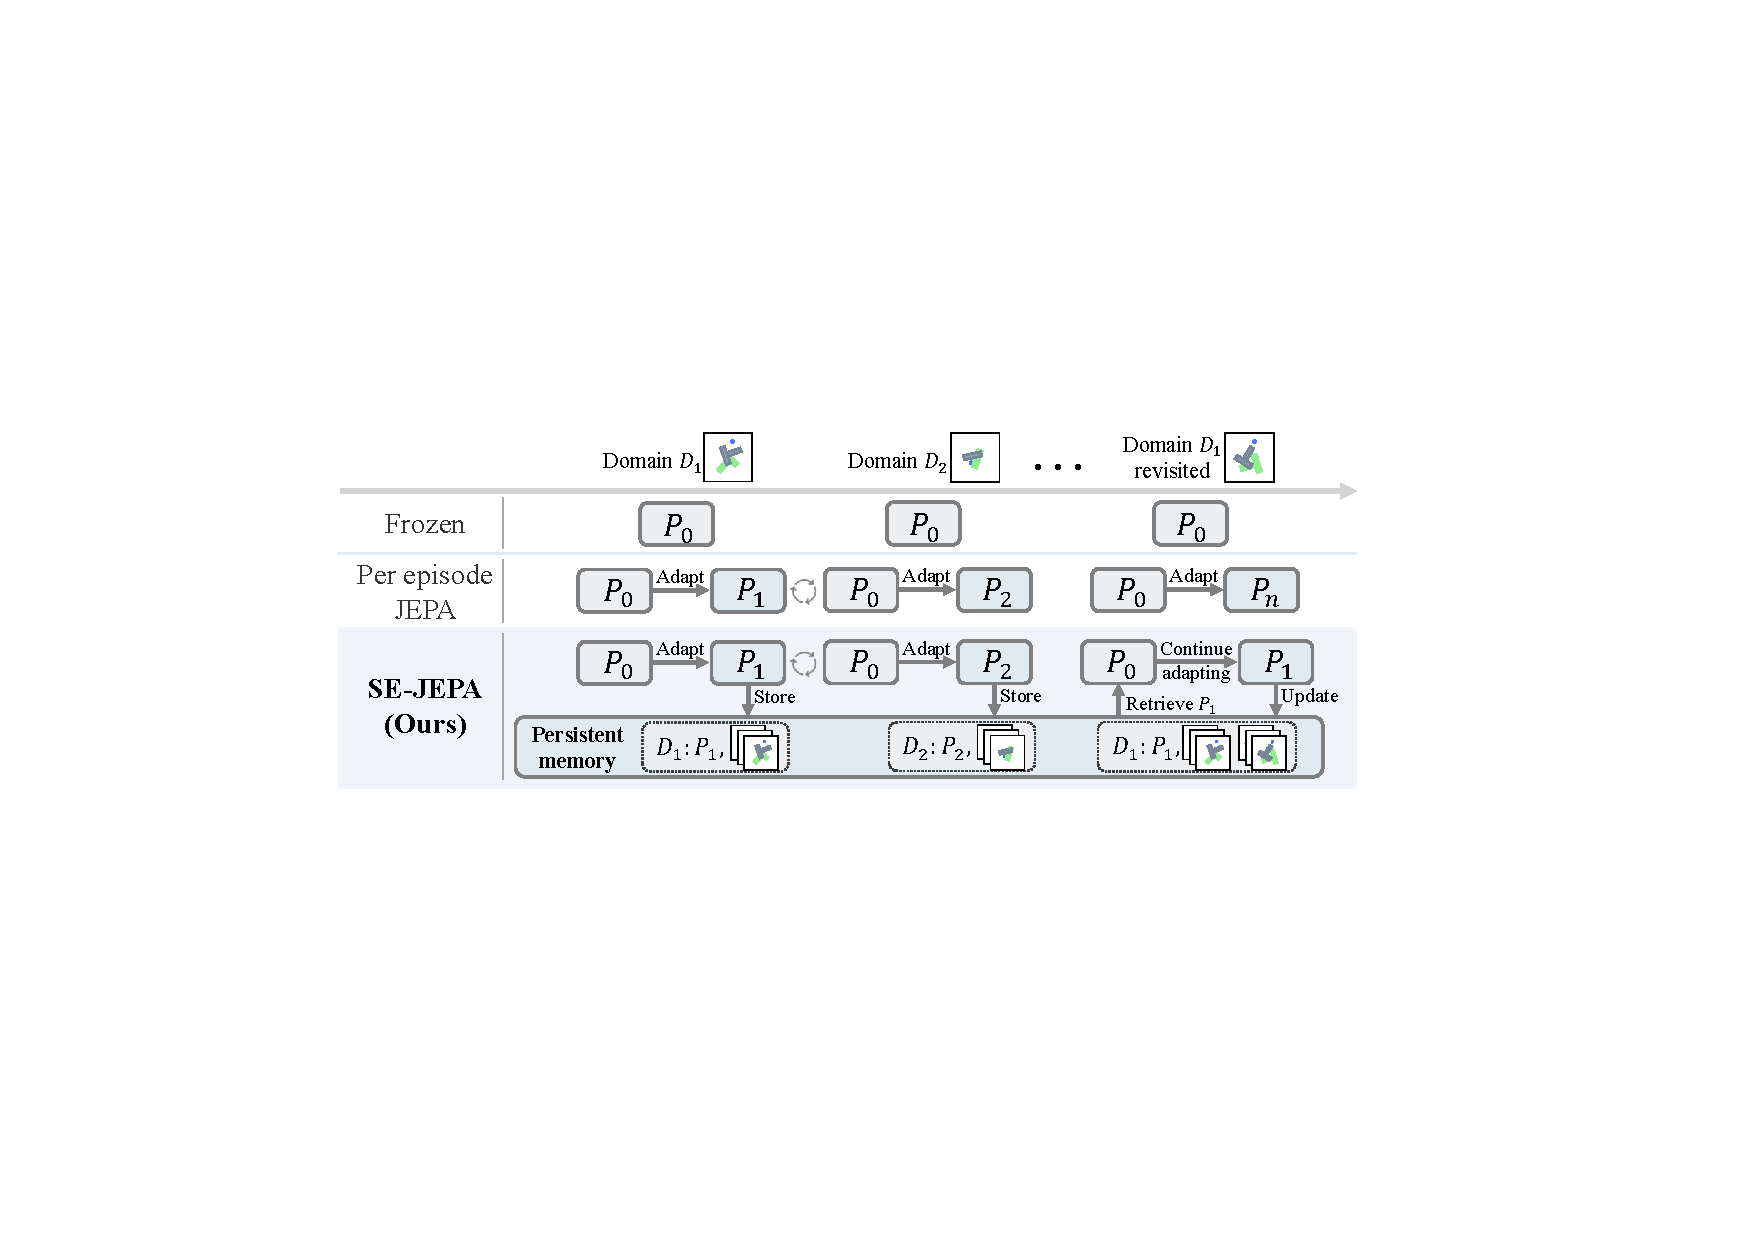
\includegraphics[width=\textwidth]{comparison.pdf}
  \caption{\textbf{From episodic adaptation to self-evolution.} A frozen world model plans every episode with the same predictor. Single-episode adaptation repairs the predictor during an episode and resets it afterwards. \ours consolidates experience into slow learners by replay and retrieves them when a shift recurs, so experience from earlier episodes can improve later planning. Domain names are for illustration; the method receives no labels.}
  \label{fig:comparison}
\end{figure*}

We introduce \ours, a self-evolving latent world model built on complementary learning systems~\cite{mcclelland1995cls}. A fast system adapts within the episode exactly as AdaJEPA does. A slow system stores the episode's transitions in the fixed latent space of the pretrained encoder and consolidates them into slow predictors by replay, one per domain that the model discovers on its own. Prediction errors and fast-update fingerprints organize this memory without domain supervision. The error of the pretrained predictor tells \ours whether an episode contains anything new. The direction of the fast update tells it which domain the experience belongs to. The error of a slow predictor on episodes it has not yet trained on tells it when that predictor can be trusted for planning. The pretrained model is never modified, so the agent can always fall back to it.

This design connects continual learning directly to visual control. With both gradient descent (GD) and the cross-entropy method (CEM), \ours improves held-out planning on PushObj shapes and PushT visual conditions (Fig.~\ref{fig:teaser_bars}). These gains use task-trained ResNet backbones; slow consolidation also improves DINO-WM on rope and granular manipulation, extending persistent learning to a different visual representation and deformable dynamics. With CEM it reaches 79.1\% success on held-out shapes and 69.9\% on unseen shapes, against 70.4\% and 54.4\% for AdaJEPA; under recoloring of the object or goal its gains exceed 27 points. Its online success improves over deployment rounds, and on deformable objects it reduces Chamfer distance by 49\% (rope) and 27\% (granular) relative to DINO-WM.

Our contributions are:
\begin{itemize}
  \setlength{\itemsep}{1pt}
  \item We identify experience replay as the bridge from episodic adaptation to persistent latent planning, motivated by a matched-stream diagnosis of weight accumulation.
  \item We propose \ours, which turns transient adaptation into lasting predictive knowledge through replay consolidation, self-discovered domains, and validation before retrieval, using prediction errors and fast-update fingerprints.
  \item We demonstrate persistent learning with task-trained ResNet and DINO-WM backbones across rigid and deformable manipulation, with higher held-out success and fewer interactions under both GD and CEM on rigid-object tasks.
\end{itemize}

\begin{figure*}[t]
  \centering
  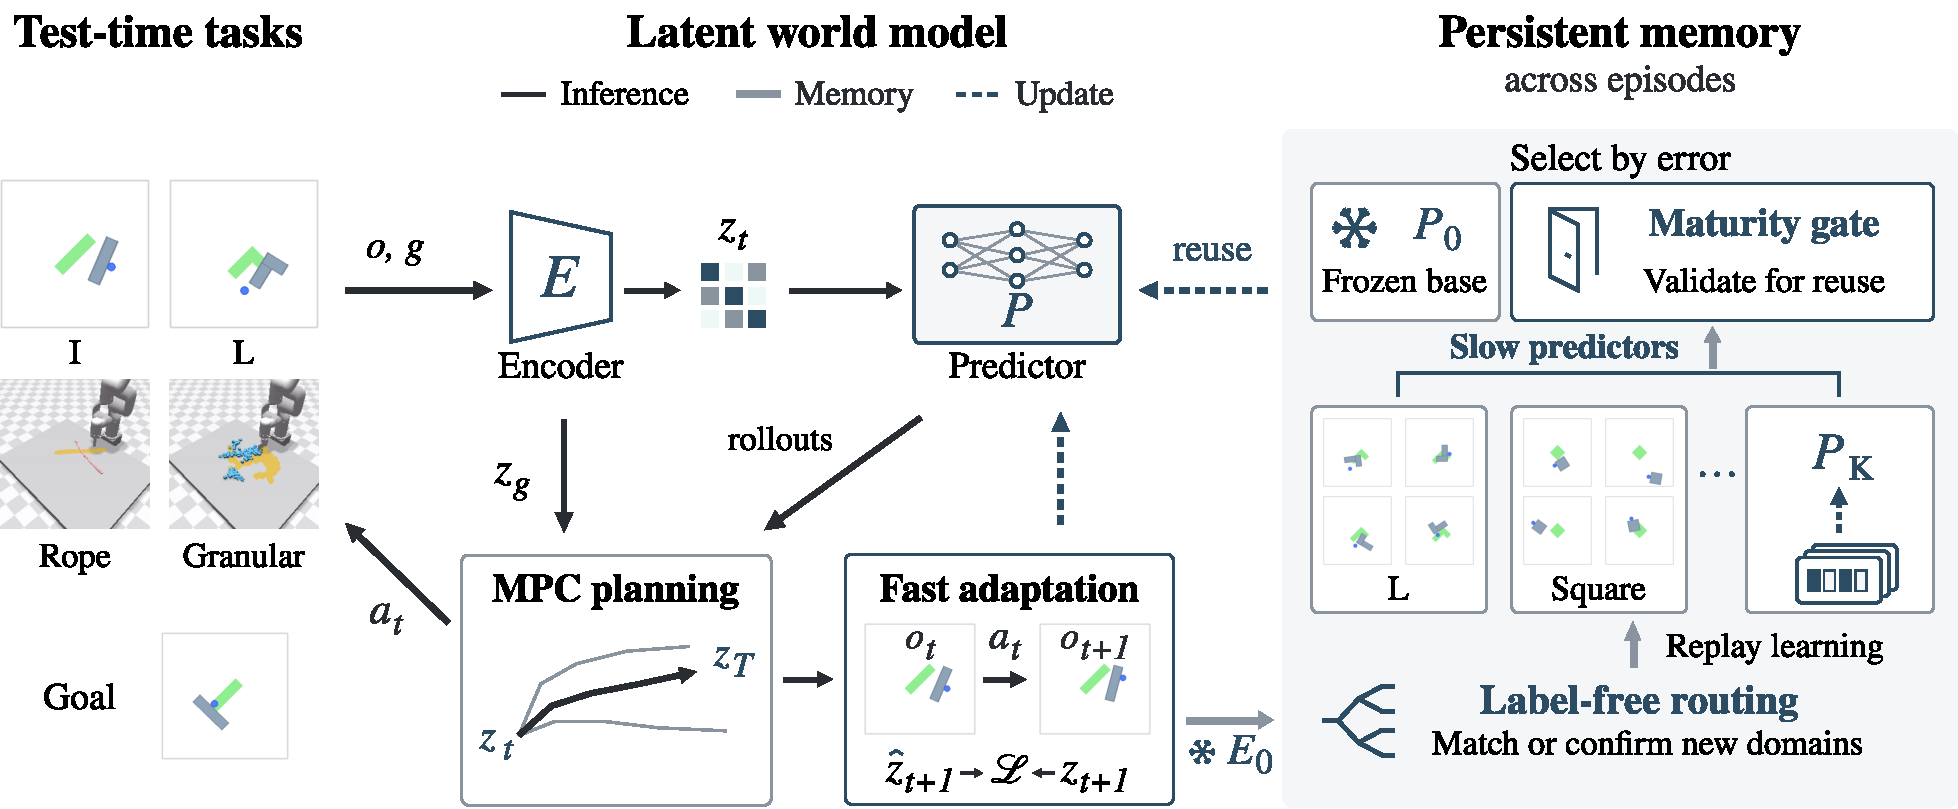
\includegraphics[width=\textwidth]{architecture.pdf}
  \caption{\textbf{\ours architecture.} The fast loop plans in latent space and adapts the predictor from observed transitions. At the end of an episode, the slow system re-encodes the trajectory with the frozen encoder, assigns unfamiliar experience to a self-discovered domain, and trains that domain's slow predictor by replay. Predictors that pass the maturity gate compete with the frozen base at the start of the next episode. Fast parameters reset at every episode; slow predictors and replay persist. Shape names illustrate memory contents and are not supervision.}
  \label{fig:architecture}
\end{figure*}

\section{Related Work}
\label{sec:related}

% \paragraph{World models for control.} World models support predictive planning~\cite{watter2015e2c,chua2018pets,hafner2019planet}, policy learning in learned simulators~\cite{ha2018worldmodels,kaiser2020simple,micheli2023iris,hafner2020dreamer,hafner2021dreamerv2,hafner2025dreamerv3}, tree search~\cite{schrittwieser2020muzero,ye2021efficientzero}, and latent control with value learning~\cite{hansen2022tdmpc,hansen2024tdmpc2}. We focus on goal-image planning, where executed actions provide transition errors for improving the deployed predictor.

% \paragraph{Predictive representations and JEPA.}Predictive learning~\cite{lecun2022path,oord2018cpc,schwarzer2021spr} complements view matching and embedding regularization~\cite{grill2020byol,zbontar2021barlow,bardes2022vicreg}. Image and video JEPA models~\cite{assran2023ijepa,bardes2024vjepa,assran2025vjepa2} build on learned visual features~\cite{caron2021dino,oquab2024dinov2,nair2022r3m}, with recent extensions to action-conditioned planning. Recent world models study feature learning, latent geometry, and separating object dynamics from visual backgrounds~\cite{zhou2024dinowm,maes2026lewm,wang2026straightening,yin2026ddpwm}. \ours uses deployment trajectories to improve planning across recurring shifts.


\noindent \textbf{World Models and Representation Learning}.
World models enable planning with learned dynamics~\cite{watter2015e2c,chua2018pets,hafner2019planet}, policy learning through imagined rollouts~\cite{ha2018worldmodels,kaiser2020simple,micheli2023iris,hafner2020dreamer,hafner2021dreamerv2,hafner2025dreamerv3}, tree search~\cite{schrittwieser2020muzero,ye2021efficientzero}, and value-guided latent control~\cite{hansen2022tdmpc,hansen2024tdmpc2}.
%
In parallel, predictive representation learning~\cite{lecun2022path,oord2018cpc,schwarzer2021spr}, non-contrastive self-supervision~\cite{grill2020byol,zbontar2021barlow,bardes2022vicreg}, and visual representation models~\cite{caron2021dino,oquab2024dinov2,nair2022r3m} have enabled learning in increasingly expressive latent spaces.
%
Building on these advances, image and video JEPA~\cite{assran2023ijepa,bardes2024vjepa,assran2025vjepa2} and action-conditioned latent world models~\cite{zhou2024dinowm,maes2026lewm,wang2026straightening,yin2026ddpwm} have advanced representation learning and predictive planning.
%
While these methods focus primarily on learning representations and dynamics, \ours{} investigates how deployment experience can be consolidated into reusable predictive knowledge across recurring distribution shifts.

\vspace{1mm}
\noindent \textbf{Test-time adaptation.}
Test-time training and entropy minimization update deployed models from unlabeled observations~\cite{sun2020ttt,wang2021tent}, including under changing distributions~\cite{wang2022cotta}. In control, each executed action supplies a target for the dynamics predictor. AdaJEPA~\cite{wang2026adajepa} uses this signal within an episode and resets the weights at its end. JEPA-TTT~\cite{zhang2026jepattt} studies a dynamics shift that persists across episodes. It trains one predictor by replaying overlapping windows from the accumulated interactions. \ours addresses recurring shifts. It keeps the pretrained weights fixed, groups compatible trajectories, and retrieves separate slow predictors whose errors on new trajectories are lower than those of the pretrained reference. These comparisons precede replay training on each trajectory.



\vspace{1mm}
\noindent\textbf{Continual Learning and Complementary Memory.}
Complementary learning systems distinguish rapid adaptation from gradual knowledge consolidation~\cite{mcclelland1995cls}.
Continual learning mitigates forgetting through experience replay~\cite{rolnick2019replay}, constrained updates~\cite{lopezpaz2017gem,kirkpatrick2017ewc}, knowledge distillation~\cite{li2016lwf}, and modular architectures~\cite{rusu2016progressive}.
In world-model planning, however, reusing a predictor directly influences subsequent actions and observations, making knowledge selection as important as retention.
% \ours{} consolidates deployment trajectories into self-discovered predictive domains, validates slow predictors on trajectories before replay training, and selects among eligible predictors and the frozen pretrained model using early-episode prediction errors.


%\vspace{1mm}
%\noindent \textbf{Continual learning and complementary memory.}
%Complementary learning systems pair rapid acquisition with slow consolidation~\cite{mcclelland1995cls}. Continual learners replay earlier experience~\cite{rolnick2019replay}, constrain updates to protect past tasks~\cite{lopezpaz2017gem,kirkpatrick2017ewc}, preserve earlier outputs through distillation~\cite{li2016lwf}, or retain separate task modules~\cite{rusu2016progressive}. In planning, predictor selection also affects subsequent actions and observations. \ours selects among validated predictors and the pretrained model using the episode's first observed transitions.

\section{SE-JEPA}
\label{sec:method}

\subsection{Motivation}
\label{sec:problem}
\label{sec:setting}
\label{sec:diagnosis}

Consider two episodes in which the agent pushes the same unfamiliar object toward different goals. The first may reveal how an off-center push rotates the object. That observation can help the agent choose a push in the second episode, even when it approaches the object from a different side. An episodic learner corrects its predictions along the first trajectory~\cite{wang2026adajepa}. Carrying its weights forward assumes that the next trajectory calls for a similar correction.

On a stream of PushObj goals, starting each episode from the preceding episode's final weights solved fewer goals than resetting the model (Appendix~D). Consecutive weight updates also point in nearly orthogonal directions (\supref{D}). A trajectory offers a different way to retain what the agent learned. Each executed action and its observed outcome provide a training example that can be revisited alongside contacts from later episodes.

\ours keeps a fast model for the current episode and trains a slow predictor on trajectories from multiple encounters (Fig.~\ref{fig:architecture}). The agent receives no labels telling it when a shape or appearance recurs. It groups trajectories by how they change the model and how well a common predictor explains them. When a new goal arrives, the first few actions provide evidence for which predictor to use.


\subsection{Fast adaptation and replay consolidation}
\label{sec:fast}
\label{sec:slow}

Each episode starts with working copies of the fixed pretrained encoder $E_0$ and predictor $P_0$. The planner minimizes latent goal cost over candidate action sequences~\cite{zhou2024dinowm,maes2026lewm} and executes the first action block. Following AdaJEPA~\cite{wang2026adajepa}, one Adam step on recent transition errors updates the predictor's last block and encoder head before replanning. These changes last only for the episode. Early replans can also retrieve a slow predictor as an \mbox{adaptation base (Sec.~\ref{sec:trust})}.

Across episodes, each \emph{predictive domain} $k$ maintains a replay buffer $\replay_k$ and slow predictor $P_{\phi_k}$. The frozen encoder re-encodes each accepted trajectory, keeping replay in a consistent latent space despite fast encoder changes. The slow predictor minimizes next-observation error on sampled replay windows:
\begin{equation}
  \loss_k(\phi_k)=
  \mathbb{E}_{(x,z^+)\sim\replay_k}
  \big\|P_{\phi_k}(x)-z^+\big\|_2^2.
  \label{eq:replay}
\end{equation}
Here $x$ contains observation embeddings and executed actions from a short history, and $z^+$ is the next observation embedding. Each slow predictor starts as a separate copy of $P_0$. Sampling windows across episodes combines different contacts and motions in the frozen representation space.

\subsection{Discovering predictive domains}
\label{sec:write}

The frozen reference first tests whether an episode contributes new experience. Let $\ell^{(0)}_{e,t}$ be its next-frame prediction error, and $\mathcal{I}_e$ index up to the first three observed transitions. Their geometric mean is
\begin{equation}
  F_e=\exp\!\left(\frac{1}{|\mathcal{I}_e|}
  \sum_{t\in\mathcal{I}_e}\log\ell^{(0)}_{e,t}\right).
  \label{eq:familiarity}
\end{equation}
If $F_e<\tau_f$, the calibrated familiarity threshold, the agent keeps $P_0$ as its adaptation base and skips the episode's direct memory write. Replay thus receives episodes the reference cannot yet predict accurately.

For an unfamiliar episode, $\Delta_e$ concatenates the fast predictor and encoder-head changes. Its normalized direction and similarity to domain $k$ are
\begin{equation}
  u_e=\frac{\Delta_e}{\|\Delta_e\|_2},
  \qquad s(e,k)=u_e^\top c_k,
  \label{eq:fingerprint}
\end{equation}
where $c_k$ is the domain's unit-length prototype. The retrieved domain is the first write candidate; otherwise, candidates are ranked by $s(e,k)$. The trajectory is assigned to a candidate domain if its predictor passes the error check in Sec.~\ref{sec:trust}. Unassigned trajectories remain in a pending pool. When a new direction aligns with those of two waiting episodes, the three trajectories establish a new domain.

Fingerprints propose candidates; prediction errors decide whether trajectories can share a learner. Delayed creation gathers evidence before fitting a new predictor. Domains merge when their predictors transfer in both directions: the larger domain retains its predictor, combines the buffers, and replays the merged experience. The frozen base remains available. Mature domains can also absorb smaller compatible groups (\supref{A}).

% Queue result displays for the next page, alongside the experiments.
% Declare experimental floats early so they accompany the results, before Conclusion.

\begin{table*}[!t]
  \centering
  \caption{\textbf{Goal-conditioned planning with CEM.} Zhou et al.~\cite{zhou2024dinowm} evaluate PushObj on two unseen shapes. Our PushObj evaluation covers seven shapes, including three unseen during pretraining. PushT covers six shifts, including three recolorings. Success is in percent. Steps is the mean replan count, with failures counted as 30. Rope and granular report Chamfer distance. Italics denote published results; bold compares the matched methods below the rule. $^{\mathrm{o}}$: offline PushT adapter; $^{\mathrm{T}}$: T-only checkpoint in our rigid-object runs.}
  \label{tab:main}
  \small
  \setlength{\tabcolsep}{3.5pt}
  \begin{tabular}{@{}lccccccccc@{}}
    \toprule
    & PushObj~\cite{zhou2024dinowm} & \multicolumn{3}{c}{PushObj (this study)} & \multicolumn{3}{c}{PushT visual shifts} & Rope & Granular\\
    \cmidrule(lr){2-2}\cmidrule(lr){3-5}\cmidrule(lr){6-8}\cmidrule(lr){9-9}\cmidrule(lr){10-10}
    Method & Unseen (2) $\uparrow$ & All (7) $\uparrow$ & Unseen (3) $\uparrow$ & Steps $\downarrow$
      & Shift (6) $\uparrow$ & Color (3) $\uparrow$ & Steps $\downarrow$ & CD $\downarrow$ & CD $\downarrow$\\
    \midrule
    \inputrows{tables/main_rows.tex}
    \bottomrule
  \end{tabular}
\end{table*}

\begin{figure*}[!t]
  \centering
  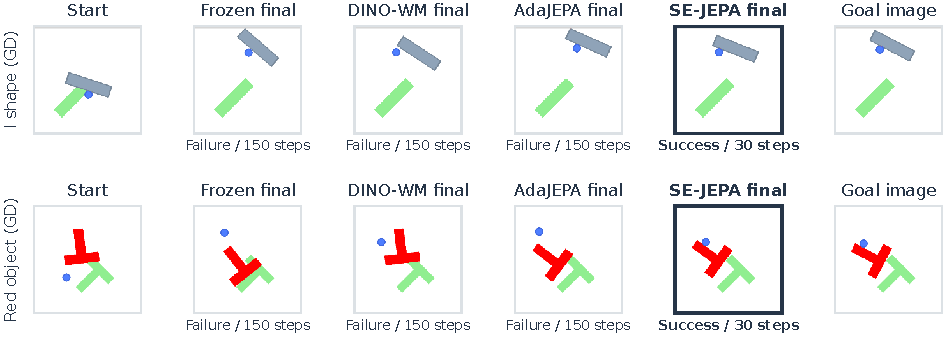
\includegraphics[width=\textwidth]{qualitative.pdf}
  \caption{\textbf{Persistent memory resolves failures of episodic adaptation.} Selected GD examples on an unseen I shape (top) and red-object shift (bottom). Frozen and AdaJEPA exhaust 30 replans in both cases; \textbf{\ours} succeeds in six and seven, respectively. Each row shares the same start and goal. The goal image specifies the pusher position and object pose; the green marker is static.}
  \label{fig:qualitative}
\end{figure*}

\begin{figure*}[!t]
  \centering
  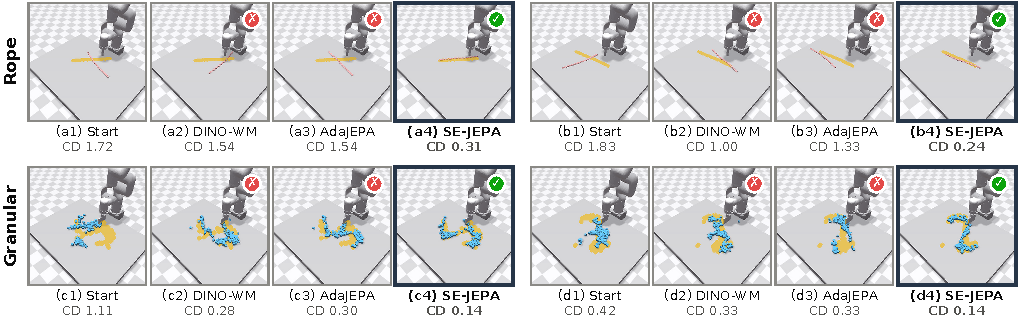
\includegraphics[width=\textwidth]{deform_qualitative.pdf}
  \caption{\textbf{Consolidated predictions support deformable manipulation.} Real FleX simulator trajectories for rope (top) and granular material (bottom), with two instances per task. Each group shows the start and the three methods' final states after 15 pushes; gold denotes the goal. These third-pass examples illustrate successful slow-only consolidation and were selected where both baselines fail. Frozen DINO-WM frames replay its executed actions. The aggregate fourth-pass results are reported in Table~\ref{tab:main}.}
  \label{fig:deform_qualitative}
\end{figure*}

\begin{figure}[!t]
  \centering
  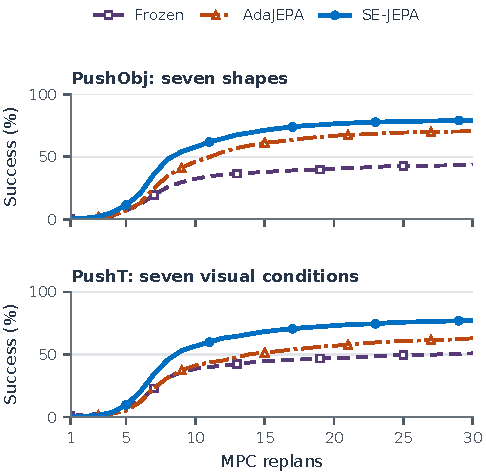
\includegraphics[width=\linewidth]{planning_efficiency.pdf}
  \caption{\textbf{Higher success within the same interaction budget.} Cumulative held-out success under CEM. Curves use all seven shapes (top) and all seven visual conditions (bottom).}
  \label{fig:efficiency_main}
\end{figure}

\begin{figure}[!t]
  \centering
  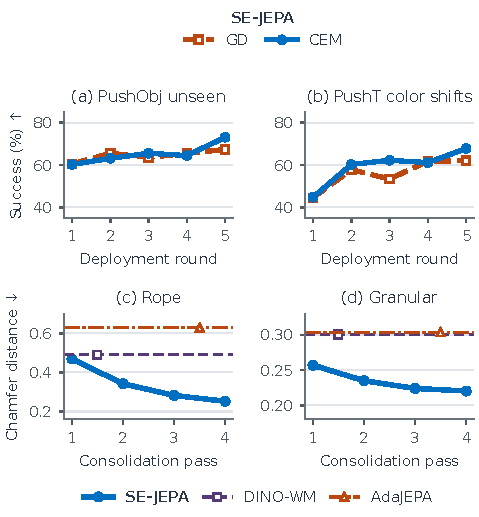
\includegraphics[width=\linewidth]{learning_progress.pdf}
  \caption{\textbf{Deployment experience improves two backbone families.} Top: ResNet-based models, with five rounds of online success on unseen PushObj shapes and three PushT color shifts; curves average three learning chains with targets resampled each round. Bottom: DINO-WM, with four consolidation passes over 50 fixed rope or granular instances; curves show mean CD. The horizontal lines are frozen DINO-WM and AdaJEPA.}
  \label{fig:deployment}
\end{figure}


\subsection{Validated retrieval for planning}
\label{sec:trust}

A slow predictor becomes eligible for planning by predicting new trajectories accurately before training on them. Before adding trajectory $\tau_e$ to a buffer, the agent rolls out the candidate predictor and the pretrained reference under the actions actually taken. Their open-loop errors in the frozen latent space give the ratio
\begin{equation}
  r_{e,k}=
  \frac{\loss_{\mathrm{roll}}(\phi_k;\tau_e)}
       {\loss_{\mathrm{roll}}(\theta_0;\tau_e)}.
  \label{eq:ratio}
\end{equation}
Here $\theta_0$ denotes the weights of $P_0$. Scoring both predictors on the same actions controls for trajectory difficulty. A write is rejected when $r_{e,k}>1.2$ in the rigid-object experiments. Accepted episodes record predictive transfer before replay training. A domain becomes eligible for retrieval when the arithmetic mean of its last three validation ratios is at most 0.9. Write acceptance admits useful experience, while the stricter maturity threshold requires consistent predictive improvement before the learner can guide planning.

During the first three replans, the agent compares eligible predictors and $P_0$ on the transitions observed so far, $\mathcal{B}_{e,t}$. It selects the predictor with the lowest recent error,
\begin{equation}
  k^\star=\argmin_{k\in\{0\}\cup\mathcal{K}_{\mathrm{eligible}}}
  \loss_{\mathrm{pred}}(\phi_k;\mathcal{B}_{e,t}),
  \qquad \phi_0=\theta_0.
  \label{eq:retrieval}
\end{equation}
The selected weights become the base of the fast predictor, preserving the corrections already made in the current episode. For an episode the reference recognizes as familiar, the base stays at $P_0$. Past trajectories therefore determine retrieval eligibility, while current observations determine which predictor guides planning.

\section{Experiments}
\label{sec:experiments}

\subsection{Setup}
\label{sec:setup}

\paragraph{Tasks.}
\emph{PushObj} has seven object shapes. Our backbone is pretrained on T, L, Z, and plus; I, square, and small tee are unseen. \emph{PushT} covers the original condition and six appearance shifts: blur, salt-and-pepper noise, darkness, and a red agent, object, or goal. \emph{Rope} and \emph{granular} manipulation use the deformable simulation of prior world-model work~\cite{zhou2024dinowm,lin2020softgym}.

\paragraph{Deployment and evaluation.}
For PushObj and PushT, \ours learns from streams of five rounds with 50 episodes per shape or condition, resampling targets every round, with three learning chains per planner. We then freeze each final memory and evaluate it on independent held-out targets: three test seeds with 50 episodes per shape or condition, whose source episodes never appear in the learning streams. For rope and granular, \ours consolidates a single slow predictor per task over four passes on 50 instances, planning with the slow predictor alone.

\paragraph{Baselines and planners.}
Frozen planning and AdaJEPA~\cite{wang2026adajepa} isolate the effect of episodic adaptation; DINO-WM~\cite{zhou2024dinowm}, LeWM~\cite{maes2026lewm}, and DDP-WM~\cite{yin2026ddpwm} compare predictive world models, and DINOv2 CLS~\cite{oquab2024dinov2} and R3M~\cite{nair2022r3m} compare visual representations. Frozen and AdaJEPA use the released task-specific checkpoints. Appendix~C records checkpoint and evaluation groups. MPC executes five actions per replan, up to 30 replans, with 100 GD steps or 10 CEM iterations of 200 samples and 30 elites.

\subsection{Remembered experience improves held-out planning}
\label{sec:sota}

Table~\ref{tab:main} places the benefit of persistent memory in the context of recent world models. The paired comparison with AdaJEPA shows gains in both success and interaction efficiency. On PushObj it reaches 79.1\% success, 8.7 points above AdaJEPA and 15 points above the best frozen world model, LeWM. The margin widens on unseen shapes, 69.9\% against 54.4\%, exactly where a fixed predictor is most wrong and remembered corrections help most. \ours also finishes faster: 13.53 replans on average against 16.02 for AdaJEPA, a 16\% reduction in interaction.

The visual shifts show the clearest gap. Averaged over six shifts, \ours reaches 76.1\% against 60.2\% for AdaJEPA. The largest gains over episodic adaptation occur under object and goal recoloring; \ours raises red-object success from 14.0\% to 47.1\% and red-goal success from 41.3\% to 68.9\%. It improves on all seven conditions, including the original one (\supref{D}).

The gains hold for gradient-based planning. With GD, \ours reaches 81.6\% on PushObj (AdaJEPA: 72.2\%) and 72.4\% on unseen shapes (55.3\%), and 75.7\% across the seven visual conditions (58.7\%), while cutting mean replans from 14.52 to 11.30 and from 17.96 to 13.21.

On deformable objects, \ours reduces Chamfer distance to 0.252 on rope and 0.220 on granular material. This is 49\% and 27\% below the DINO-WM model it builds on, with the lowest reported CD among the methods in Table~\ref{tab:main}. Fast adaptation is switched off in this setting, so the improvement comes entirely from consolidated knowledge.

Remembered experience also makes each interaction more productive (Fig.~\ref{fig:efficiency_main}). The cumulative success curves show how the benefit develops across the planning budget, complementing the mean replan counts in Table~\ref{tab:main}.

\subsection{Qualitative results}
\label{sec:qualitative}

Figure~\ref{fig:qualitative} contrasts selected episodes in which persistent memory changes the outcome. On the unseen I shape, \ours reaches the goal in six replans; under object recoloring, it succeeds in seven. Frozen and AdaJEPA fail within the 30-replan budget in both cases. The red-object example makes the difference visible: the baselines leave the T-shaped object at the wrong orientation, whereas \ours brings it into the goal pose. Additional complete trajectories appear in \supref{E}.

Figure~\ref{fig:deform_qualitative} extends the behavioral evidence to deformable objects. The consolidated predictor brings the rope and particles toward the target configuration using slow memory without within-episode adaptation. This complements the aggregate CD reductions: deployment experience improves the physical outcomes that the planner reaches.

\subsection{Stronger with deployment}
\label{sec:deployment}

Figure~\ref{fig:deployment} tracks knowledge accumulation during deployment, with new targets in every round. With CEM, unseen-shape success rises from 60.2\% in the first round to 73.1\% in the fifth, and success over the seven visual conditions from 67.1\% to 79.0\%. GD follows the same trend, from 60.4\% to 67.3\% and from 69.1\% to 75.8\%.

Deformable manipulation shows the same behavior (Fig.~\ref{fig:deform_passes}). Rope CD falls from 0.469 after the first pass to 0.252 after the fourth, and granular CD from 0.257 to 0.220, with both curves well below the pretrained DINO-WM. The knowledge also transfers to new instances: a rope predictor saved after the first pass, frozen and tested on 91 unseen instances, lowers CD from 0.664 to 0.349.

% Keep every main-paper table and figure before the closing section.
\FloatBarrier
% Keep the closing section together when the preceding column is nearly full.
\Needspace{18\baselineskip}
\section{Conclusion}
\label{sec:conclusion}

\ours makes deployment experience reusable through selective trajectory storage, replay, and validated predictor retrieval. With task-trained ResNet models, it improves held-out success and replan efficiency under GD and CEM, and continues learning across 14 recurring shape and appearance domains with one memory. With DINO-WM, slow consolidation reduces deformable goal error, and a rope predictor trained in one pass transfers to new instances.

\paragraph{Future work.}
Longer histories, diagnostic pushes, and better near-goal action ranking may improve planning.


% Mandatory for CVPR 2027: after the main text, before the references; not counted toward the page limit.
% Flush remaining figures and reset both column heights before references.
\clearpage
\onecolumn
\twocolumn
\raggedbottom
\section*{LLM Usage Statement}
Large language models (OpenAI Codex and Anthropic Claude) were used to draft and revise substantial portions of the manuscript text, and to assist with literature and source checks, LaTeX organization, figure generation, and result aggregation. They also assisted with experimental code, including offline world-model adapters and experiment orchestration. All quantitative results are taken from saved experimental outputs or explicitly cited published sources; language-model output is not used as experimental evidence. The authors take full responsibility for the claims, citations, code, and final verification of the manuscript.


{
    \small
    % Keep bibliography endings substantial without altering entry wording.
    \let\standardthebibliography\thebibliography
    \renewcommand{\thebibliography}[1]{%
      \standardthebibliography{#1}%
      \tolerance=1000\relax
      \setlength{\parfillskip}{0pt plus 0.25\linewidth}%
    }
    \bibliographystyle{ieeenat_fullname}
    \bibliography{references}
}

% ---------------------------------------------------------------------------
% Appendix appended for whole-paper review (2026-11-05). For submission, the
% same sections also build standalone from supplement.tex.
% ---------------------------------------------------------------------------
\clearpage
\flushbottom
\appendix
\twocolumn[{\centering{\Large\bfseries Supplementary Material\par}\vspace{1.2em}}]
\section{Implementation and Memory Management}
\label{app:implementation}

\paragraph{Compute environment.}
Model training and evaluation were conducted on systems equipped with $8\times$ NVIDIA GeForce RTX 5090 GPUs and $8\times$ NVIDIA A100 GPUs.

\subsection{Fast and slow learning}
The label-free rigid-object configuration builds on the episodic adaptation loop of AdaJEPA~\cite{wang2026adajepa}. At every replan, recent observed transitions provide a self-supervised next-state prediction loss. The predictor's last block and the encoder's designated projection/head parameters are adapted with one Adam step. The episode-local predictor and encoder changes are reset at the next episode. A retrieved slow predictor supplies the predictor initialization; it does not replace the frozen reference encoder.

Persistent replay is re-encoded by the reference encoder. Each slow learner is a full predictor copy, initialized from the pretrained predictor rather than from the final fast parameters of the episode that created the domain. For each slow optimization step, up to eight stored episodes are sampled with replacement; each contributes a random window of up to six latent frames. The prediction objective averages one-step observation-feature errors over the available history windows. Actions condition the prediction; the loss is computed only on observation features. Standard writes use 15 Adam steps. Founding a learner after $n$ stored episodes uses $15n$ steps to process the accumulated evidence. Merging likewise adds replay updates for absorbed experience.

\begin{table}[t]
  \centering
  \caption{Label-free configuration used for PushObj and PushT. The seven-round stream in Appendix~D uses a slow learning rate of $2\times10^{-4}$ for all replay updates.}
  \label{tab:hyperparams}
  \small
  \begin{tabular}{lr}
    \toprule
    Setting & Value\\
    \midrule
    Fast predictor learning rate & $5\times10^{-4}$\\
    Fast encoder-head learning rate & $10^{-5}$\\
    Fast steps per replan & 1\\
    Recent adaptation buffer & 5 transitions\\
    Slow learning rate & $10^{-4}$\\
    Slow steps per standard write & 15\\
    Slow batch size (episodes) & 8\\
    Slow sampled window (frames) & up to 6\\
    Familiarity threshold $\tau_f$ & 0.0146\\
    Existing-domain cosine threshold & 0.10\\
    New-domain cosine threshold & 0.05\\
    Episodes to confirm a domain & 3\\
    Pending-pool capacity & 40\\
    Minimum episodes to train a learner & 3\\
    Retrieval window & first 3 replans\\
    Maturity history length $m$ & 3\\
    Maturity error-ratio threshold $\tau_m$ & 0.9\\
    Write rejection ratio & 1.2\\
    Merge evidence per direction & 2 episodes\\
    Merge relative tolerance & 0.5\\
    Fragment absorption interval & 25 episodes\\
    Absorption error-ratio threshold & 0.8\\
    Fragment-size limit & $<6$ episodes\\
    \bottomrule
  \end{tabular}
\end{table}

Replay stores compact latent trajectories rather than images. The pending pool is bounded, and merging and absorption remove redundant predictor copies as compatible domains are recognized.

\subsection{Order of decisions}
Algorithm~\ref{alg:sejepa} summarizes a learning episode. Familiarity uses the geometric mean of newest-frame prediction errors on up to the first three observed transitions. The threshold is calibrated once on the shape backbone and transfers unchanged to the visual experiments.

\begin{algorithm}[t]
\caption{One deployment-learning episode of \ours}
\label{alg:sejepa}
\begin{algorithmic}[1]
  \Require Frozen $(E_0,P_0)$, memory $\memory$, initial observation $o$, goal $g$
  \State Reset fast parameters to $(E_0,P_0)$
  \State Initialize recent buffer $\mathcal{B}$ and episode trajectory $\tau$
  \While{budget remains and task is not complete}
    \State Optimize an action sequence with the current fast model
    \State Execute its first block; observe the next state
    \State Append real transitions to $\mathcal{B}$ and $\tau$
    \If{within the early retrieval window}
      \State Form candidates: $P_0$ and mature slow predictors
      \State Restrict to $P_0$ if the observed episode is familiar
      \State Select the smallest observed prediction error
      \State Load the selected predictor, retaining the fast offset
    \EndIf
    \State Adapt the fast model on recent real transitions
  \EndWhile
  \State Encode $\tau$ with frozen $E_0$
  \State Measure pre-update rollout errors of existing predictors
  \If{episode is unfamiliar}
    \State Propose a domain using retrieval or an update fingerprint
    \State Reject an incompatible write, or retain pending evidence
    \If{a domain is assigned or newly confirmed}
      \State Record validation before replay training when a learner exists
      \State Append latent experience; update its slow predictor
      \State Check bidirectional merges and periodic absorption
    \EndIf
  \EndIf
  \State Discard episode-local fast parameters
\end{algorithmic}
\end{algorithm}

The selected predictor's error is evaluated before it learns from the current episode, so maturity reflects transfer to data the predictor has not fitted. In read-only evaluation, the episode-end write, validation-history update, slow training, merging, and absorption steps are all disabled.

\subsection{Fingerprints and delayed domain founding}
A fingerprint concatenates the adapted predictor and encoder-head changes and is normalized to unit length. Domain prototypes accumulate normalized fingerprints from episodes planned from the reference; episodes starting from a slow predictor do not redefine that reference-based prototype. If an episode retrieved a slow predictor, its trajectory is first considered for that predictor's domain, subject to the error-ratio check before replay. Otherwise, it tries compatible domain directions in descending cosine order.

An unassigned episode enters a pending pool. It confirms a new domain when at least two pending fingerprints align with its own above the new-domain threshold. These members need not be pairwise aligned with one another; the incoming fingerprint is the common reference for this confirmation. The members and the new episode are transferred together to the new replay. No ground-truth shape or appearance category participates in this procedure.

\subsection{Merging and fragment absorption}
For a new unfamiliar episode, every existing trained learner is evaluated before training. The resulting ratios provide cross-domain evidence. Let $G_{A\to B}$ be the geometric mean error ratio of learner $B$ on recent episodes assigned to $A$, and $G_{A\to A}$ the corresponding ratio for learner $A$. Domains merge only if both directions satisfy
\begin{equation}
 G_{A\to B}\leq \min\{1,(1+\epsilon_m)G_{A\to A}\},
\end{equation}
with the symmetric condition for $B\to A$. Each direction requires two jointly evaluated episodes in the primary configuration. The larger domain retains its learner and incorporates the union of stored experience. Identifiers of merged domains remain retired for the rest of the stream.

Every 25 episodes, small immature domains can be absorbed into a mature predictor that explains their experience with an error ratio at most 0.8. The primary configuration limits absorption to fragments with fewer than six episodes and fewer than three maturity measurements. Pending-pool absorption and the additional absolute-error gate are disabled in the shape and visual experiments.

\section{Evaluation Protocols}
\label{app:protocols}

\subsection{Shape shifts}
The shape learning stream has five deployment rounds over seven shapes, with 50 episodes per shape in every round. The held-out benchmark uses target seeds 2000, 2100, and 2200, each with 350 episodes. I, square, and small tee are unseen in pretraining; T, L, Z, and plus are seen.

Each planner has three learned memory states. Every state is evaluated on all three held-out seeds; for each seed we average over episodes and states, and standard deviations are computed over the three seed-level means. The CEM states are S7t3, S7t3b, and S7t3s700, where S7t3b is a rerun of S7t3 that replaces a run in which no learner matured. Frozen and AdaJEPA use the same three held-out seeds; the external baselines use seed 2000.

\subsection{Visual shifts}
The paired visual evaluation contains the original T condition, blur, salt-and-pepper noise, darkness, red agent, red object, and red goal. Three five-round learning chains resample targets every round, with 350 episodes per round. Held-out testing uses three target seeds and 50 episodes per condition. Direct checks of source-episode identifiers confirm that held-out sources never occur in the learning streams and that the three test seeds use disjoint sources.

The color-learning curve in Fig.~\mainref{fig:deployment} aggregates red-agent, red-object, and red-goal episodes. For each round and learning chain, it sums successes over the three conditions and divides by 150 episodes, then reports the mean and sample standard deviation of the three chain-level rates. The three conditions share the same 50 source targets within a chain and round.

The external visual baselines use the established VIS50 collection with planning seed 100. The external comparisons use its six shifted conditions, with 50 paired initial/goal states per condition.

\subsection{Success and interaction counts}
Rigid-object success follows the environment's goal test: object-position error below 20 simulator units and angular error below $\pi/9$. Each executed model action contains five physical actions, and an episode has at most 30 MPC replans. For episode $i$ with success indicator $S_i$ and first successful replan $T_i$,
\begin{equation}
  \overline{T} = \frac{1}{N}\sum_{i=1}^{N}
  \big[\, S_i T_i + (1-S_i)\, T_{\max} \big], \qquad T_{\max}=30.
\end{equation}
Equivalently, $\overline{T} = T_{\max} - \sum_{t=1}^{T_{\max}-1} F(t)$, where $F(t)$ is the fraction of episodes solved by replan $t$; the cumulative curves in Fig.~\mainref{fig:efficiency_main} visualize $F$.

\subsection{Deformable manipulation}
Rope and granular each use one slow predictor, a DINO-WM backbone, and 50 instances revisited over four passes, with the same targets, order, and planning seeds in every pass. The slow-only variant plans from the slow predictor without fast within-episode updates. CEM uses 300 samples, 30 elites, and 10 iterations, with three MPC iterations of five pushes each. The unseen-rope evaluation freezes the predictor saved after the first pass and tests it on 91 instances absent from the learning stream, against the frozen reference on the same instances. Two frozen granular episodes with unstable batched particle simulation were rerun individually with identical settings and seeds.

\begin{table*}[t]
 \centering
 \caption{Both planners on the paired held-out sets. Shape All and Unseen use held-out PushObj targets. Visual All averages seven conditions and Shift six; visual Steps averages all seven conditions.}
 \label{tab:planners}
 \small
 \begin{tabular}{llcccccc}
 \toprule
 & & \multicolumn{3}{c}{PushObj} & \multicolumn{3}{c}{PushT}\\
 \cmidrule(lr){3-5}\cmidrule(lr){6-8}
 Planner & Method & All $\uparrow$ & Unseen $\uparrow$ & Steps $\downarrow$ & All $\uparrow$ & Shift $\uparrow$ & Steps $\downarrow$\\
 \midrule
 \inputrows{tables/paired_planners.tex}
 \bottomrule
 \end{tabular}
\end{table*}

\section{Baseline Checkpoints and Comparisons}
\label{app:baselines}

\paragraph{Predictive world models.}
The comparisons focus on latent world models used for visual planning: DINO-WM, LeWM, and DDP-WM, with DINO CLS and R3M as representation baselines. Frozen and AdaJEPA use released task-specific checkpoints. For PushObj and PushT, \ours uses ResNet-based world models trained directly on task trajectories. Its PushObj backbone is trained for three epochs on 16,000 trajectories covering T, L, Z, and plus. The additional DINO-WM shape model uses the same training trajectory count and epoch budget, with 4,000 validation trajectories and batch size 32. DINO CLS and R3M use existing T-only checkpoints; LeWM and DDP-WM use their corresponding checkpoint adapters.

\paragraph{Offline generative baselines.}
For PushT we use offline-trained DreamerV3 and IRIS predictors for CEM planning and evaluate them on the same VIS50 targets as DINO-WM. Their published PushObj results use two unseen shapes and a goal test on both the agent and the object~\cite{zhou2024dinowm}; those scores do not measure our three-unseen-shape metric. We leave their PushObj cells unreported.

\paragraph{Evaluation groups.}
The paired Frozen/AdaJEPA/\ours comparison uses the independent held-out target sets in Appendix~B. External visual baselines use VIS50, with 50 initial/goal pairs in each of six shifted conditions and planning seed 100. The table separates these evaluation groups. Within each group, methods receive the same targets and planning budget. PushT Shift averages blur, noise, dark, red agent, red object, and red goal; Color averages the last three. The original condition is included in the seven-condition tables and curves, but excluded from Shift.

\paragraph{Deformable results.}
The rope and granular experiments use DINO-WM with pretrained DINOv2 patch features as the frozen backbone. This complements the task-trained ResNet setting used for rigid-object manipulation. AdaJEPA adapts within each episode, whereas \ours uses a consolidated slow predictor. Italic CD entries for DreamerV3, IRIS, R3M, and DINO CLS come from the ten-instance evaluation of Zhou et al.~\cite{zhou2024dinowm}. Our frozen DINO-WM reference uses the same 50 instances as our deformable adaptation runs and appears in both the DINO-WM and Frozen rows. The repeated-instance and unseen-rope protocols are specified in Appendix~B.

\section{Additional Results}
\label{app:additional}

\subsection{All object shapes}
Table~\ref{tab:shape_domains} reports every held-out shape. \ours gives the largest gains on the unseen shapes: with GD, I rises from 44.7\% (AdaJEPA) to 77.6\% and square from 46.7\% to 61.1\%. It also leads on the seen shapes in aggregate.

\begin{table*}[t]
 \centering
 \caption{Held-out success (\%) per PushObj shape. I, square, and small tee are unseen in pretraining. All averages the seven shapes.}
 \label{tab:shape_domains}
 \small
 \begin{tabular}{llcccccccc}
 \toprule
 Planner & Method & I & L & Square & Z & Small tee & Plus & T & All\\
 \midrule
 \inputrows{tables/shape_domains.tex}
 \bottomrule
 \end{tabular}
\end{table*}

\subsection{All visual conditions}
Table~\ref{tab:visual_domains} and Fig.~\ref{fig:visual_gains} break the paired visual results down by condition. \ours improves on all seven conditions with both planners. The largest gains, more than 25 points, appear under red-object and red-goal recoloring, where episodic adaptation has to rediscover the new appearance in every episode.

\begin{table*}[t]
 \centering
 \caption{Held-out visual success (\%) per condition on the paired targets. All averages seven conditions; Shift excludes Original.}
 \label{tab:visual_domains}
 \small
 \begin{tabular}{llccccccccc}
 \toprule
 Planner & Method & Original & Blur & Noise & Dark & Red agent & Red object & Red goal & All & Shift\\
 \midrule
 \inputrows{tables/visual_domains.tex}
 \bottomrule
 \end{tabular}
\end{table*}

\begin{figure*}[t]
 \centering
 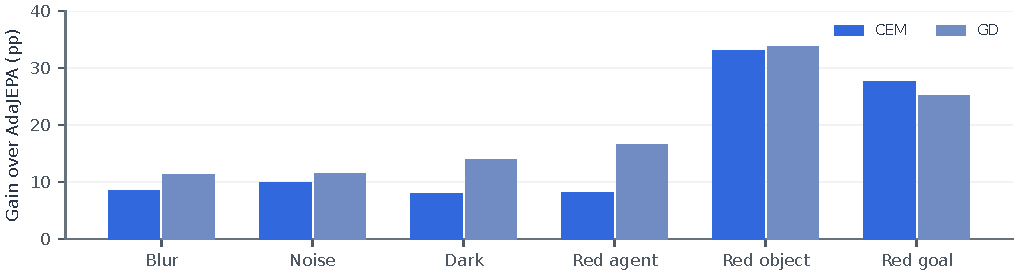
\includegraphics[width=\textwidth]{visual_gains.pdf}
 \caption{Held-out gain of \textbf{\ours} over AdaJEPA for each visual shift, in percentage points.}
 \label{fig:visual_gains}
\end{figure*}

\subsection{Planning efficiency}
Figure~\mainref{fig:efficiency_main} plots cumulative held-out success against the number of MPC replans. \ours pulls ahead within the first four replans and keeps the lead for the rest of the budget, showing how the advantage develops before the final 30-replan evaluation.



\subsection{Deformable manipulation}


Figure~\mainref{fig:deployment} shows the four-pass learning curves in the main paper. Table~\ref{tab:deform} adds standard errors to the deformable results of Table~\mainref{tab:main}. Table~\ref{tab:deform_passes} follows consolidation pass by pass at two slow learning rates. With $10^{-4}$, CD decreases at every pass on both tasks. With $2\times10^{-4}$, rope improves faster in the early passes and both rates reach a similar level after four passes, so consolidation is robust to the learning rate.

\begin{table}[t]
  \centering
  \caption{Deformable manipulation: mean CD $\pm$ standard error over 50 instances. \ours uses its slow predictor after four passes.}
  \label{tab:deform}
  \small
  \begin{tabular}{lcc}
    \toprule
    Method & Rope CD $\downarrow$ & Granular CD $\downarrow$\\
    \midrule
    \inputrows{tables/deform_rows.tex}
    \bottomrule
  \end{tabular}
\end{table}

\begin{table}[t]
  \centering
  \caption{CD of \ours after each consolidation pass at two slow learning rates (mean $\pm$ standard error, 50 instances).}
  \label{tab:deform_passes}
  \footnotesize
  \setlength{\tabcolsep}{2.5pt}
  \begin{tabular}{ccccc}
    \toprule
    & \multicolumn{2}{c}{lr $10^{-4}$} & \multicolumn{2}{c}{lr $2\times10^{-4}$}\\
    \cmidrule(lr){2-3}\cmidrule(lr){4-5}
    Pass & Rope & Granular & Rope & Granular\\
    \midrule
    \inputrows{tables/deform_passes.tex}
    \bottomrule
  \end{tabular}
\end{table}

\subsection{A seven-round shape stream}
A second PushObj stream runs seven rounds with a slow learning rate of $2\times10^{-4}$, one chain per planner. Each round has 50 episodes per shape, drawn without replacement and excluding the held-out sources, for 2{,}450 episodes per planner. Online success rises from 70.6\% in the first round to 78.6\% in the seventh with GD, and from 72.3\% to 78.3\% with CEM.

The episode logs record the fast-update fingerprint of every episode. Figure~\ref{fig:directions} shows the cosine between consecutive fingerprints: the mean is 0.018 for both planners, and most of the mass lies near zero. These measurements support consolidating transition data rather than accumulating episode-specific parameter updates (Sec.~\mainref{sec:diagnosis}). Over the stream, \ours writes 622 (GD) and 663 (CEM) episodes to memory, 25.4\% and 27.1\% of all episodes, and finishes 630 and 666 episodes with a slow predictor.

\begin{figure*}[t]
 \centering
 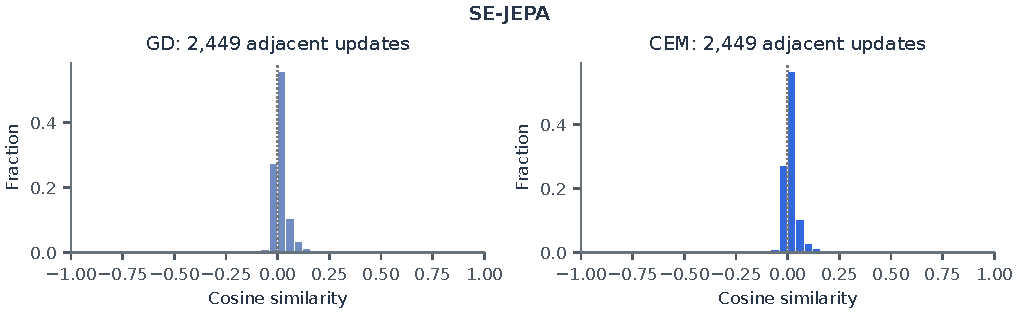
\includegraphics[width=\textwidth]{update_directions.pdf}
 \caption{Cosine similarity between consecutive fast-update fingerprints in the seven-round shape stream (2{,}449 pairs per planner).}
 \label{fig:directions}
\end{figure*}

\subsection{What \ours chooses to learn}
\label{sec:selectivity}

\ours learns selectively. In a seven-round PushObj stream of 2{,}450 episodes per planner, it writes only 25\% (GD) to 27\% (CEM) of episodes to memory; the rest are familiar to the pretrained model, still pending, or rejected by validation. Retrieval is just as targeted: slow predictors plan about one episode in four, and the reference handles the rest.

Selective writing leaves familiar dynamics to the pretrained model, which \ours never overwrites. On the four pretraining shapes, \ours reaches 86.0\% held-out success with CEM and 88.4\% with GD, against 82.3\% and 84.8\% for AdaJEPA. This preserves a useful pretrained reference while allowing specialized predictors to add capacity for recurring shifts.

\section{Qualitative Examples and Reproducibility}
\label{app:qualitative}

\subsection{Full trajectories}
Figure~\mainref{fig:qualitative} selects an unseen-I and a red-object episode where both baselines fail and \ours succeeds under GD. These illustrate changes in planning behavior; aggregate success is evaluated on the complete held-out sets. The source package supplies the first held-out target of test seed 2000 for each condition, and the displayed conditions are chosen by outcome. All methods share identical initial and goal observations. The panels use a consistent crop size to enlarge the movable objects, with every colored foreground element preserved.

Figures~\ref{fig:full_shape} and~\ref{fig:full_visual} provide additional CEM examples on the first held-out target of the same test seed: an unseen square and a red-agent shift. They show the complete trajectories and each method's prediction loss. These are separate from the GD examples in the main paper.

\begin{figure*}[!t]
 \centering
 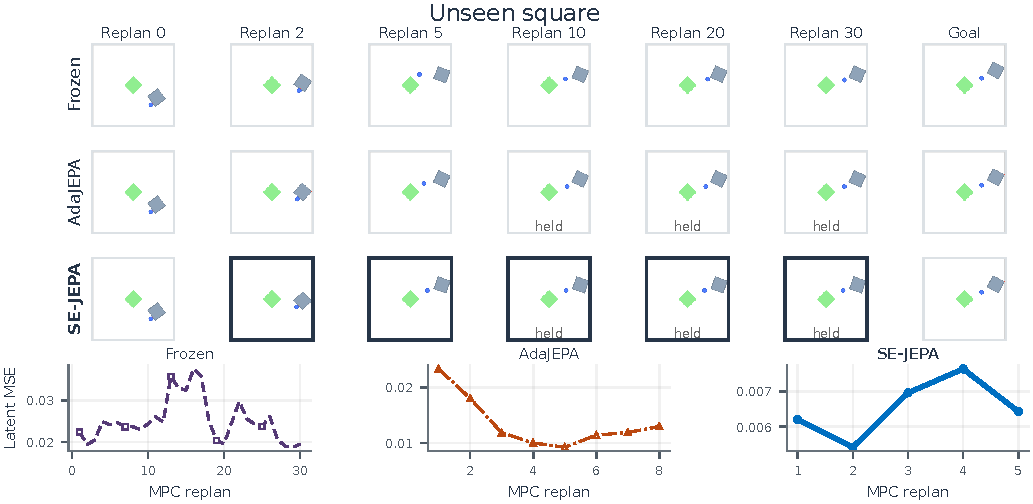
\includegraphics[width=\textwidth]{shape_full.pdf}
 \caption{Full unseen-square example with intermediate frames and prediction-loss traces. Frames marked held repeat the terminal state after success. \textbf{\ours} reaches the goal at replan five, AdaJEPA at replan eight, and the frozen model does not succeed within the budget.}
 \label{fig:full_shape}
\end{figure*}

\begin{figure*}[!t]
 \centering
 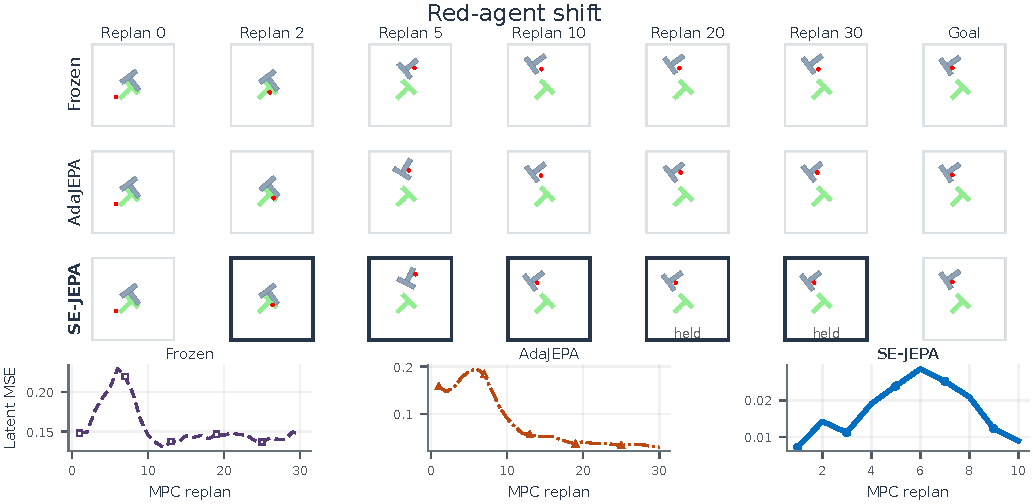
\includegraphics[width=\textwidth]{visual_full.pdf}
 \caption{Full red-agent example, replayed in the original simulator from the executed actions. \textbf{\ours} succeeds at replan ten; Frozen and AdaJEPA reach the 30-replan limit.}
 \label{fig:full_visual}
\end{figure*}

Each loss curve is measured in the latent space of its own model, so it describes how prediction error evolves within a method over the episode. Task success, judged in the shared simulator state, is the common yardstick across methods.

\subsection{Deformable rollout sequences}
Figures~\ref{fig:full_rope} and~\ref{fig:full_granular} expand the four deformable examples from Fig.~\mainref{fig:deform_qualitative}. Each row shows the start, every third push, and the goal over the same 15-push budget. The instances were selected from the repeated 50-instance learning stream where both baselines fail and the consolidated predictor succeeds. These third-pass examples illustrate slow-only planning; the aggregate results in Table~\mainref{tab:main} use the fourth pass. DINO-WM frames replay its recorded actions in the original FleX simulator. AdaJEPA and \ours frames were saved during planning, and the displayed CD values come from the original evaluation logs.

\begin{figure*}[p]
 \centering
 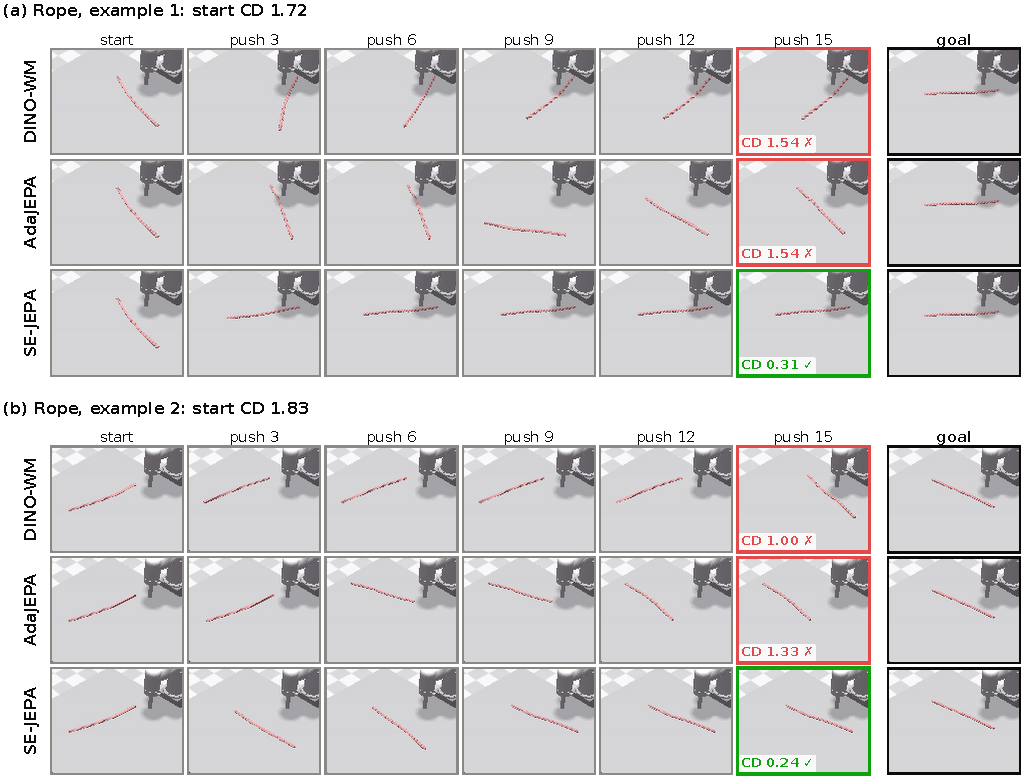
\includegraphics[width=\textwidth]{rope_full.pdf}
 \caption{\textbf{Complete rope manipulation sequences.} Two real instances, with DINO-WM, AdaJEPA and \ours sharing the initial state and goal. Columns show pushes 0, 3, 6, 9, 12 and 15, followed by the goal. Lower final Chamfer distance (CD) is better; the final-frame markers report task success. \ours uses the third-pass slow predictor without within-episode adaptation.}
 \label{fig:full_rope}
\end{figure*}

\begin{figure*}[p]
 \centering
 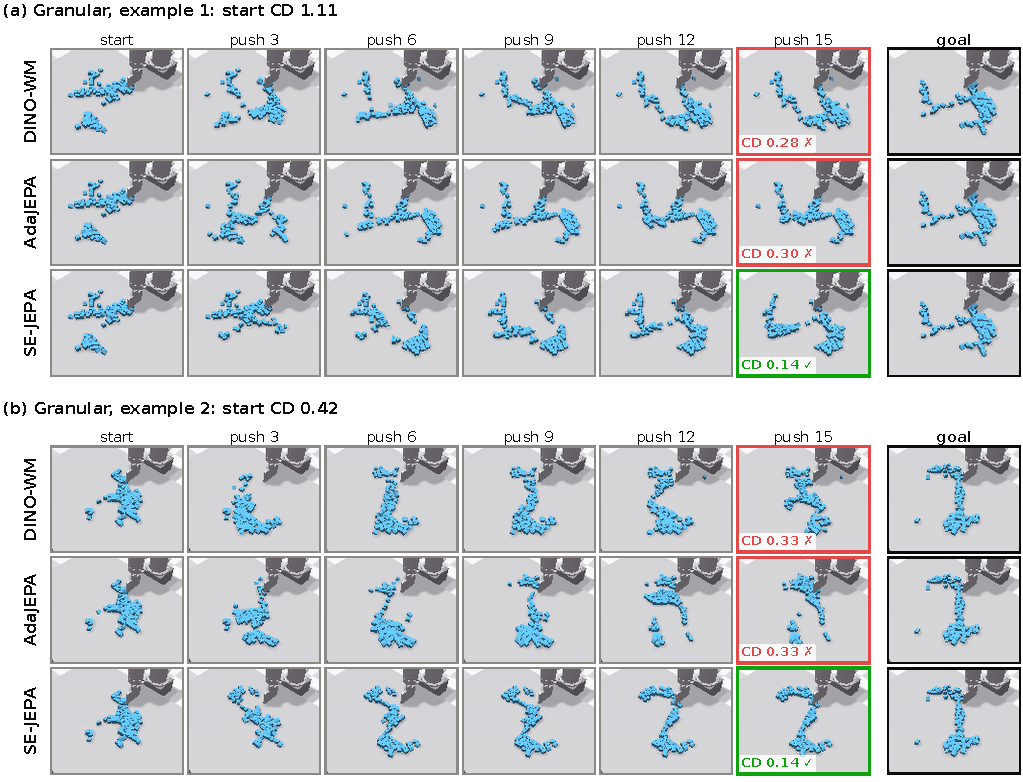
\includegraphics[width=\textwidth]{granular_full.pdf}
 \caption{\textbf{Complete granular manipulation sequences.} Two real instances under the same 15-push budget and reporting convention as Fig.~\ref{fig:full_rope}. All simulator frames are retained from the archived execution or action replay; the labels report recorded final CD and success. The third-pass slow predictor guides \ours.}
 \label{fig:full_granular}
\end{figure*}

\subsection{Reproducibility}
Tables and plots use the bundled reporting snapshot and the archived Drive experiment packages. The revised trajectory panels are rendered directly from the packages' simulator frames; the asset manifest records their source files and hashes. Success and Steps are computed from the final episode files and their run configurations. Offline world-model checkpoints record the upstream code revision, the epoch budget, the model configuration, and hashes of the adapter sources. Code, configurations, and learned memory states will be released.


\end{document}
